\documentclass[12pt,a4paper]{article}
\usepackage[utf8]{inputenc}
\usepackage[russian]{babel}
\usepackage[OT1]{fontenc}
\usepackage{amsmath}
\usepackage{amsfonts}
\usepackage{amssymb}
\usepackage{graphicx}

\newcommand{\x}{\ensuremath{x}}
\newcommand{\xx}[1]{\ensuremath{\x_{#1}}}
\newcommand{\M}{\ensuremath{M}}
\newcommand{\MM}[1]{\ensuremath{\M_{#1}}}
\newcommand{\customint}{\ensuremath{\int}}
\newcommand{\customdx}{\ensuremath{\,\mathrm{d}\x}}

\begin{document}
\begin{center}\LARGE\bf
Task Solver.
\end{center}

\tableofcontents

\section{Общие сведения}

\textbf{Task Solver} --- проект по созданию программного средства для автоматизированного решения математических задач с подробным решением.

Большинство заданий по элементарной и высшей математике требует применения стандартных и достаточно формализованных действий, которые могут быть выполнены компьютерной программой. Разработка такой программы и является целью проекта. Окончательное название проекта еще не выбрано. Task Solver --- это рабочее название, которым мы в дальнейшем будем пользоваться.

На данный момент существует единственный способ воспользоваться возможностями проекта --- через электронную почту. Проект развивается на некоммерческой основе, поэтому у разработчиков нет возможности организовать постоянно работающий сервер.

Все вопросы, предложения и замечания можно присылать на электронную почту
\begin{verbatim}
tasksolver.maintenance@gmail.com
\end{verbatim}
Если вы хотите, чтобы в проект была добавлена возможность решения какой-либо задачи, то, чтобы это произошло с большей вероятностью и большей скоростью, нужно прислать, кроме формулировки самой задачи, всю необходимую теорию и несколько примеров решения.

\section{Решение заданий по электронной почте}

Передать задания для решения можно через электронную почту. Взаимодействие осуществляется просто: пользователь посылает письмо с кодом для генерации решений и получает в ответном письме приложенный \textit{pdf}-файл с текстом решений.

Письмо с кодом можно посылать на один из следующих почтовых адресов:
\begin{verbatim}
psb0vlml@gmail.com
\end{verbatim}
Обработка писем, поступивших на электронную почту, будет производиться по возможности как можно чаще. Разработчики постараются гарантировать обработку писем не реже одного раза каждый будний день.

Темой письма обязательно должна быть строка 
\begin{verbatim}
SolvePlease
\end{verbatim}
без пробелов, без других символов, в точности такая, с учетом регистра. Иначе письмо будет воспринято как спам и удалено!

Вот пример того, как должно выглядеть письмо на сайте mail.ru:
\begin{center}
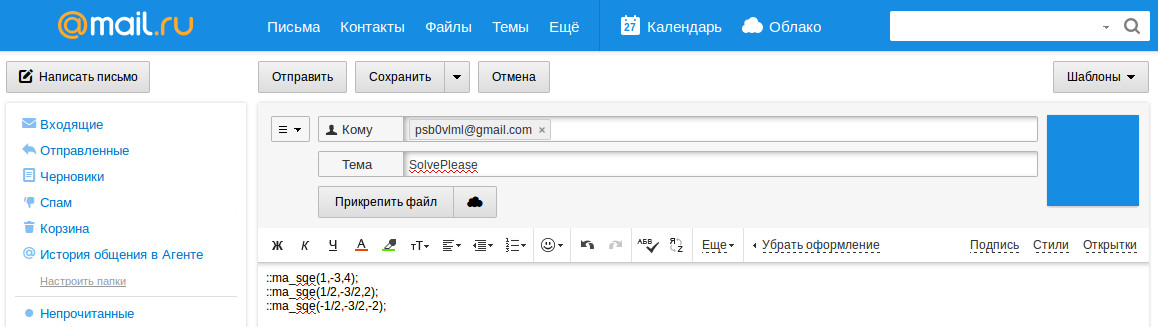
\includegraphics[width=130mm]{ts-email-desc-img1.jpg} 
\end{center}

\section{Правила записи математических выражений}

Правила ввода чисел точно такие, как и для многих других подобных программ. Целая и дробная часть десятичных дробей разделяются символом «\texttt{.}» (точка). Перед отрицательными числами ставится знак «\texttt{-}» (минус). Числитель и знаменатель обыкновенных дробей разделяется при помощи символа «\texttt{/}» (прямой слэш).

Если при вычислениях встретится число с плавающей точкой, то результат вычислений также будет числом с плавающей точкой. Числа с плавающей точкой округляются до четырёх разрядов после запятой.

Обозначения арифметических операций ничем не отличаются от классического представления, используются математические знаки: «\texttt{+}», «\texttt{-}», «\texttt{*}», «\texttt{/}». 

Возведение в степень можно обозначать тремя способами: «\texttt{\^{ }}», «\texttt{\^{ }\^{ }}», «\texttt{**}». 

Извлечение корня степени $n$ записывают, как степень \texttt{\^{ }(1/n)}. нахождение факториала числа обозначается восклицательным «\texttt{!}» знаком. Для увеличения приоритета операции, как и в математике, при записи команд используют круглые «\texttt{()}» скобки.

Можно использовать достаточно большой набор математических функций. Следует иметь ввиду, что некоторые
названия функций отличаются от названий, используемых в отечественной литературе: Вместо tg --- \texttt{tan}, вместо ctg --- \texttt{cot}, вместо arcsin --- \texttt{asin}, вместо arccos --- \texttt{acos}, вместо arctg --- \texttt{atan}, вместо arcctg --- \texttt{acot}, вместо ln --- \texttt{log}, вместо cosec --- \texttt{csc}. 

\noindent\begin{tabular}{||c|c||c|c||}
\hline 
Функция & Команда & Функция & Команда \\ 
\hline 
Синус ($\sin$) & \texttt{sin} & Гиперболический синус ($\sh$) & \texttt{sinh}\\ 
\hline 
Тангенс ($\tg$) & \texttt{tan} &Гиперболический тангенс ($\th$) & \texttt{tanh}\\ 
\hline 
Арксинус ($\arcsin$) & \texttt{asin} & Арккосинус ($\arccos$) & \texttt{acos} \\ 
\hline 
Арктангенс ($\arctg$) & \texttt{atan} & Арккотангенс ($\arcctg$) & \texttt{acot} \\ 
\hline 
Секанс ($\sec$) & \texttt{sec} & Гиперболический секанс ($\mathop{sech}$) & \texttt{sech}\\ 
\hline 
Косинус ($\cos$) & \texttt{cos} & Гиперболический косинус ($\ch$) & \texttt{cosh} \\ 
\hline 
Котангенс ($\ctg$) & \texttt{cot} & Гиперболический котангенс ($\cth$) & \texttt{coth} \\ 
\hline 
Косеканс ($\cosec$) & \texttt{csc} & Гиперболический косеканс ($\mathop{csch}$) & \texttt{cosh} \\ 
\hline 
 &  &  Квадратный корень ($\sqrt{\ }$) & \texttt{sqrt}\\ 
\hline 
 &  &  Натуральный логарифм ($\ln$) & \texttt{log}\\
\hline 
\end{tabular} 

Для записи функции необходимо указать ее название, а затем, в круглых
скобках записать через запятую значения аргументов.

Одним из самых сложных занятий является запись сложных выражений, содержащих степени, дроби и другие конструкции, в линейной форме (в текстовой форме записи, при помощи ASCII символов, в одну строку).

Для облегчения данного процесса нелишне дать несколько рекомендаций:

1. Не забывайте ставить знак умножения! По правилам математики удвоенное значение переменной \texttt{х} записывается в виде $2x$, но команда должна выглядеть как \texttt{2*x}.

2. В случае сомнения всегда лучше поставить «лишние», дополнительные скобки (). Числитель и знаменатель выражения всегда необходимо заключать в скобки. А также при возведении в степень основание и степень лучше всегда брать
в скобки.

3. Функция не существует отдельно от своих аргументов (если таковые имеются). Поэтому, например, при возведении в степень можно взять всю функцию с аргументами в скобки, а потом уже возводить полученную конструкцию в нужную степень: математическое выражение $\sin^2x$ должно быть записано как \texttt{(sin(x))**2}.

4. Также помните, что несколько аргументов функции записываются в скобках, через запятую.

5. Недопустима запись функции \texttt{sin(2*x)} в виде \texttt{sin*2*x} или \texttt{sin2x}.

6. В случае записи сложного выражения разбейте его на несколько простых составляющих, введите их по отдельности, а затем объедините, используя рассмотренные ранее обозначения введенных команд.

\section{Доступные для решения задания}
Информация справедлива для версии 0.0.191

\subsection{Найти скалярное произведение двух векторов}

\noindent \textbf{Команда для почты:} \mbox{ mg\_vsp }

\noindent \textbf{Текст задания:} Найти скалярное произведение векторов $\vec{v}$ и $\vec{w}$

\noindent \textbf{Аргументы команды:}\\ $v$ --- последовательность значений, первое из которых есть целое число, определяющее количество следующих за ним значений; каждое это  значение должно быть действительным числом;\\
$w$ --- последовательность значений, первое из которых есть целое число, определяющее количество следующих за ним значений; каждое это  значение должно быть действительным числом;\\
 

\noindent \textbf{Пример команды:} ::\mbox{ mg\_vsp }($3$, $11$, $12$, $13$, $3$, $24$, $25$, $26$);

\subsection{Найти длину вектора}

\noindent \textbf{Команда для почты:} \mbox{ mg\_vl }

\noindent \textbf{Текст задания:} Найти длину вектора $vec{v}$

\noindent \textbf{Аргументы команды:}\\ $v$ --- последовательность значений, первое из которых есть целое число, определяющее количество следующих за ним значений; каждое это  значение должно быть действительным числом;\\
 

\noindent \textbf{Пример команды:} ::\mbox{ mg\_vl }($3$, $10$, $11$, $12$);

\subsection{Найти математическое ожидание и дисперсию непрерывной случайной величины, заданной функцией плотности вероятности}

\noindent \textbf{Команда для почты:} \mbox{ mc\_crvdfdev }

\noindent \textbf{Текст задания:} Найти математическое ожидание и дисперсию непрерывной случайной величины, заданной функцией плотности вероятности $f(\x)$ на промежутке $a<x<b$ (равной нулю в остальных точках).

\noindent \textbf{Аргументы команды:}\\ $f(\x)$ ---  Значение должно быть функцией; Значение должно быть выражением, содержашим только x в качестве переменной;\\
$a$ ---  Значение должно быть действительным числом;\\
$b$ ---  Значение должно быть действительным числом;\\
 

\noindent \textbf{Пример команды:} ::\mbox{ mc\_crvdfdev }($x$, $0$, $1$);

\subsection{Найти математическое ожидание непрерывной случайной величины, заданной функцией плотности вероятности}

\noindent \textbf{Команда для почты:} \mbox{ mc\_crvdfev }

\noindent \textbf{Текст задания:} Найти математическое ожидание непрерывной случайной величины, заданной функцией плотности вероятности $f(\x)$ на промежутке $a<x<b$ (равной нулю в остальных точках).

\noindent \textbf{Аргументы команды:}\\ $f(\x)$ ---  Значение должно быть функцией; Значение должно быть выражением, содержашим только x в качестве переменной;\\
$a$ ---  Значение должно быть действительным числом;\\
$b$ ---  Значение должно быть действительным числом;\\
 

\noindent \textbf{Пример команды:} ::\mbox{ mc\_crvdfev }($x$, $0$, $1$);

\subsection{Найти определенный интеграл}

\noindent \textbf{Команда для почты:} \mbox{ mm\_dint }

\noindent \textbf{Текст задания:} Найти определенный интеграл $\int^b_a f(\x)d\x$.

\noindent \textbf{Аргументы команды:}\\ $f(\x)$ ---  Значение должно быть функцией; Значение должно быть выражением, содержашим только x в качестве переменной;\\
$a$ ---  Значение должно быть действительным числом;\\
$b$ ---  Значение должно быть действительным числом;\\
 

\noindent \textbf{Пример команды:} ::\mbox{ mm\_dint }($sin(x)+x$, $0$, $1$);

\subsection{Найти неопределенный интеграл}

\noindent \textbf{Команда для почты:} \mbox{ mm\_iint }

\noindent \textbf{Текст задания:} Найти неопределенный интеграл $\int f(\x)d\x$.

\noindent \textbf{Аргументы команды:}\\ $f(\x)$ ---  Значение должно быть функцией; Значение должно быть выражением, содержашим только x в качестве переменной;\\
 

\noindent \textbf{Пример команды:} ::\mbox{ mm\_iint }($sin(x)+x$);

\subsection{Решение системы линейных уравнений 3 на 3 методом Крамера}

\noindent \textbf{Команда для почты:} \mbox{ ma\_slesk33 }

\noindent \textbf{Текст задания:} Решить систему линейных уравнений методом Крамера $$\left\{\begin{array}{l}a_{11}\cdot x_{1}+a_{12}\cdot x_{2}+a_{13}\cdot x_{3}=b_{1},\\a_{21}\cdot x_{1}+a_{22}\cdot x_{2}+a_{23}\cdot x_{3}=b_2,\\a_{31}\cdot x_{1}+a_{32}\cdot x_{2}+a_{33}\cdot x_{3}=b_{3}.\end{array}\right.$$

\noindent \textbf{Аргументы команды:}\\ $a_{11}$ ---  Значение должно быть действительным числом;\\
$a_{12}$ ---  Значение должно быть действительным числом;\\
$a_{13}$ ---  Значение должно быть действительным числом;\\
$a_{21}$ ---  Значение должно быть действительным числом;\\
$a_{22}$ ---  Значение должно быть действительным числом;\\
$a_{23}$ ---  Значение должно быть действительным числом;\\
$a_{31}$ ---  Значение должно быть действительным числом;\\
$a_{32}$ ---  Значение должно быть действительным числом;\\
$a_{33}$ ---  Значение должно быть действительным числом;\\
$b_{1}$ ---  Значение должно быть действительным числом;\\
$b_{2}$ ---  Значение должно быть действительным числом;\\
$b_{3}$ ---  Значение должно быть действительным числом;\\
 

\noindent \textbf{Пример команды:} ::\mbox{ ma\_slesk33 }($11$, $12$, $13$, $21$, $22$, $23$, $31$, $32$, $33$, $-1$, $-2$, $-3$);

\subsection{Найти определитель матрицы 3 на 3}

\noindent \textbf{Команда для почты:} \mbox{ ma\_mdet33 }

\noindent \textbf{Текст задания:} Найти определитель матрицы $\begin{pmatrix} a_{11} & a_{12} & a_{13} \\ a_{21} & a_{22} & a_{23} \\ a_{31} & a_{32} & a_{33} \end{pmatrix}$

\noindent \textbf{Аргументы команды:}\\ $a_{11}$ ---  Значение должно быть действительным числом;\\
$a_{12}$ ---  Значение должно быть действительным числом;\\
$a_{13}$ ---  Значение должно быть действительным числом;\\
$a_{21}$ ---  Значение должно быть действительным числом;\\
$a_{22}$ ---  Значение должно быть действительным числом;\\
$a_{23}$ ---  Значение должно быть действительным числом;\\
$a_{31}$ ---  Значение должно быть действительным числом;\\
$a_{32}$ ---  Значение должно быть действительным числом;\\
$a_{33}$ ---  Значение должно быть действительным числом;\\
 

\noindent \textbf{Пример команды:} ::\mbox{ ma\_mdet33 }($1$, $2$, $3$, $4$, $5$, $6$, $7$, $8$, $9$);

\subsection{Найти обратную матрицу 3 на 3}

\noindent \textbf{Команда для почты:} \mbox{ ma\_minv33 }

\noindent \textbf{Текст задания:} Найти обратную матрицу для матрицы $\begin{pmatrix} a_{11} & a_{12} & a_{13} \\ a_{21} & a_{22} & a_{23} \\ a_{31} & a_{32} & a_{33} \end{pmatrix}$

\noindent \textbf{Аргументы команды:}\\ $a_{11}$ ---  Значение должно быть действительным числом;\\
$a_{12}$ ---  Значение должно быть действительным числом;\\
$a_{13}$ ---  Значение должно быть действительным числом;\\
$a_{21}$ ---  Значение должно быть действительным числом;\\
$a_{22}$ ---  Значение должно быть действительным числом;\\
$a_{23}$ ---  Значение должно быть действительным числом;\\
$a_{31}$ ---  Значение должно быть действительным числом;\\
$a_{32}$ ---  Значение должно быть действительным числом;\\
$a_{33}$ ---  Значение должно быть действительным числом;\\
 

\noindent \textbf{Пример команды:} ::\mbox{ ma\_minv33 }($1$, $2$, $3$, $4$, $5$, $6$, $7$, $8$, $9$);

\subsection{Решение квадратного уравнения}

\noindent \textbf{Команда для почты:} \mbox{ ma\_sqe }

\noindent \textbf{Текст задания:} Решить квадратное уравнение $a\cdot x^2+b\cdot x+c=0$.

\noindent \textbf{Аргументы команды:}\\ $a$ ---  Значение должно быть действительным числом; Значение должно быть не равно нулю;\\
$b$ ---  Значение должно быть действительным числом;\\
$c$ ---  Значение должно быть действительным числом;\\
 

\noindent \textbf{Пример команды:} ::\mbox{ ma\_sqe }($1$, $0$, $0$);



\end{document}